\documentclass[unicode, notheorems, minimal, nologo, handout]{beamer}
\usetheme[numbers, totalnumbers]{Statmod}
% If you have more than three sections or more than three subsections in at least one section,
% you might want to use the [compress] switch. In this case, only the current (sub-) section
% is displayed in the header and not the full overview.
%\mode<presentation>
%{
%  
%
%  \setbeamercovered{transparent}
%  \beamertemplatenavigationsymbolsempty
%  % or whatever (possibly just delete it)
%}

\mode<handout> {
    \usepackage{pgfpages}
    \setbeameroption{show notes}
    \pgfpagesuselayout{2 on 1}[a4paper, border shrink=5mm]
}

%\usepackage{pscyr}
\usepackage[T2A]{fontenc}
\usepackage[utf8]{inputenc}
\usepackage[russian]{babel}
\usepackage{amsthm}
\usepackage{pdfpages}
\usepackage{bibentry}

\usepackage{natbib}   % omit 'round' option if you prefer square brackets
\bibliographystyle{plainnat}

\graphicspath{{fig/}}

%\usepackage{tikz}
% you only need this when using TikZ graphics

\newtheorem{theorem}{Теорема}
\newtheorem{example}{Пример}
\newtheorem{definition}{Определение}


\DeclareMathOperator*{\E}{\mathrm{E}}
\DeclareMathOperator*{\D}{\mathrm{D}}
\DeclareMathOperator*{\sign}{sign}
\DeclareMathOperator*{\argmin}{arg\,min}
\DeclareMathOperator*{\Int}{Int}
\DeclareMathOperator*{\err}{err}
\newcommand\norm[1]{\left\lVert#1\right\rVert}
\newcommand\abs[1]{\left\lvert#1\right\rvert}


\title[Оптимальные планы для оценивания производных]{ Оптимальные планы для оценивания производных в полиномиальной регрессионной модели без свободного члена}

%\author{Барсуков Егор Вячеславович, гр. 16-Б.04мм}
%\institute[СПбГУ]{
%    Санкт-Петербургский государственный университет \\
%    Математико-Механический факультет \\
%    Кафедра статистического моделирования \\
%   \vspace{1.25cm}
%    Преддипломная практика
%}
%
%\date{
%	Санкт-Петербург \\
%    2020 г.
%}

%\subject{Beamer}
% This is only inserted into the PDF information catalog. Can be left
% out.

% Delete this, if you do not want the table of contents to pop up at
% the beginning of each subsection:
% \AtBeginSubsection[]
% {
%   \begin{frame}<beamer>
%     \frametitle{Outline}
%     \tableofcontents[currentsection,currentsubsection]
%   \end{frame}
% }

\institute[Санкт-Петербургский Государственный Университет]{
    \small
    Санкт-Петербургский государственный университет\\
    Прикладная математика и информатика\\
    Вычислительная стохастика и статистические модели\\
    \vspace{1.25cm}
    Преддипломная практика}

\date[Защита]{Санкт-Петербург, 2020}

\subject{Talks}

\begin{document}


\begin{frame}
    \titlepage
    \note {
    Тема работы --- Оптимальные планы для оценивания производных в полиномиальной регрессионной модели без свободного члена. Работа выполнена на кафедре статистического моделировния. Научный руководитель д.ф.-м.н., профессор В. Б. Мелас.
    }
\end{frame}

\section{Постановка задачи}

\begin{frame}
	\frametitle{Уравнение регрессии}
	\begin{equation*}
		y_j = \theta^\top f(x_j) + \varepsilon_j, \quad j = 1 \ldots N, \, x_j \in \mathcal{X}
	\end{equation*}
	\begin{itemize}
		\item $N$ --- количество экспериментов;
		\item $f(x)$ --- вектор регрессионных функций;
		\item $\theta = (\theta_1, \ldots, \theta_m)^\top$ --- неизвестные параметры;
		\item $x_1, \ldots, x_N$ --- условия проведения эксперимента;
		\item $\mathcal{X}$ --- множество планирования;
		\item $\varepsilon_1, \ldots, \varepsilon_N$ --- случайные величины, характеризующие ошибки наблюдений.
		\begin{itemize}
			\item Несмещенные $\mathbb{E} \varepsilon_i = 0$
			\item Некоррелированные $\mathbb{E} \varepsilon_i \varepsilon_j = 0$ для $i \neq j$
			\item Равноточные $\mathbb{E} \varepsilon_i^2 = \sigma^2$ для всех $i$
		\end{itemize}
	\end{itemize}
	
	\note{
	Для того, чтобы сформулировать задачу введем несколько определений. Пусть задано уравнение регрессии, c количеством экспериментов $N$ и количеством параметров $n$ на некотором множестве планирования $\mathcal{X}$ с несмещенными (средним ноль) некоррелированными равноточными (с одинаковой дисперсией) ошибками.
	}
\end{frame}

\begin{frame}
	\frametitle{План эксперимента и информационная матрица}
	\begin{definition}
	Планом эксперимента называется следующая дискретная вероятностная мера
		\begin{equation*}
			\xi = 
				\begin{pmatrix}
				x_1 & \ldots & x_m \\
				\omega_1 & \ldots & \omega_m
			\end{pmatrix}, \quad x_i \in \mathcal{X}.
		\end{equation*}
	\end{definition}
	 
  	\begin{definition}
		Для плана эксперимента определим его информационную матрицу
		\begin{equation*}
			M(\xi) = \int_{\mathcal{X}} f(x) f^\top(x) \xi (dx).
  		\end{equation*}
	\end{definition}
  	
	\note {
	Для такого уравнения регрессии определим план эксперимента, то есть дискретную вероятностную меру носитель которой сосредоточен на множестве планирования. Далее носитель этой меры будет называться опорными точками плана, а соостветствующие вероятности --- весами этих опорным точек.
	
	При практическом применении (когда возможно проводить только целое количество измерений) в точке $x_i$ проводят приблизительно $N/\omega_i$ измерений так, чтобы всего было проведено $N$ измерений.
	
	Для планов эксперимента также определим информационную матрицу следующим образом.

}
	
\end{frame}

\begin{frame}
	\frametitle{C-оптимальный план эксперимента}
	\begin{definition}
		C-оптимальным планом эксперимента для данного вектора $c$ называется план минимизирующий функцию $\Phi$
		\begin{equation*}
				\Phi(\xi) = \begin{cases}
				c^\top M(\xi)^{-} c, \quad \text{если } \exists v \text{, такой, что } \; c = M(\xi) v\\
				+\infty, \quad  \text{иначе}
		    \end{cases},
		\end{equation*}
		где $M(\xi)^{-}$ --- псевдообратная матрица к информационной матрице плана
	\end{definition}
	
	\begin{itemize}
		\item C-оптимальный план минимизирует дисперсию МНК-оценки~$\theta^\top c$;
		\item В общем виде задача нахождения таких планов не решена
	\end{itemize}
	
	\note{
	В этой работе изучены с-оптимальные планы, которые определены как минимум показанного здесь функционала для некоторого вектора $c$.
	
	Важной особенностью таких планов, которая дает им практическую ценность, является то, что они минимизируют оценку по методу наименьших квадратов значения $\theta^\top c$.
	
	Явных решений в общем виде для произвольного $c$ не существует, но изучаются некоторые важные частные случаи (например $c = f(z)$). Рассмотрение одного из таких случаев и является одной из целей этой работы.
	}
\end{frame}

\begin{frame}
	\frametitle{Постановка задачи}
	\begin{definition}
	Если $c = f'(z) = \left(f'_1(z), \ldots, f'_m(z) \right)^\top$ то соответствующий план называется планом для оценки производной в точке $z$.
	\end{definition}
	\begin{itemize}
		\item Целью работы является описание оптимальных планов для оценки производной в модели $f(x) = \left(x, \ldots, x^m \right)$ при носителе $\mathcal{X} = [0, d]$.
		\item Это имеет практический смысл, если существует априорное знание о значении функции в нулевой точке и эксперимент проводится на положительном отрезке.
		\item Решение задачи отличается от того, которое получается при носителе, границе которого не принадлежит ноль, которое описано в \citep{melasmain}.
		\item Разработать алгоритм численно решающий задачу нахождения c-оптимальных планов для произвольного $c$.
	\end{itemize}
	
	\note{
	Если вектор $c$ составлен из значений производных компонент вектора $f$ в некоторой точке $z$, то такой план называется планом для оценки производной в точке $z$.
	
	В силу сказанного на предыдущем слайде свойства с-оптимальных планов такой план минимизирует дисперсию оценки производной функции $\theta^\top f(x)$ в точке $z$.
	
	В работе будет рассматриваться полиномиальная модель без нулевого члена, при этом множество планирования --- положительный отрезок с началом в нуле.
	
	Такая модель имеет смысл, когда рассматривается зависимость некоторого значения от параметра, определенного только на положительной полуоси. При этом с известным значением в точке 0. Простым примером такой зависимости может являться зависимость расстояния от времени.
	
	Также целью работы является построение алгоритма для численного нахождения с-оптимальных планов в общем случае.
	} 
	
\end{frame}

\section{План для оценки производной на положительном отрезке}

\begin{frame}
	\frametitle{Теорема Элвинга \citep{melas2010}}
	\begin{theorem}
	Допустимый план $\xi^\star$ с носителем $x_1, \ldots, x_m \in \mathcal{X}$ и весами $\omega_1, \ldots, \omega_m$ является $c$-оптимальным тогда и только тогда, когда существует $p \in \mathbb{R}^k$ и константа $h$ такие, что выполняются следующие условия:
  \begin{subequations}
  \label{eq:elfving}
  \begin{align}
	&\abs{p^\top f(x_i)} = 1 &&i=1..m \leqslant n, \\
	&\abs{p^\top f(x)} \leqslant 1  &&x \in \mathcal{X}, \\
	&c = h \sum_{i=1}^m \omega_i f(x_i) p^\top f(x_i) .
  \end{align}
  Кроме того,
  \begin{equation*}
  	h^2 = c^\top M^{-}(\xi^{*})c.
  \end{equation*}
  \end{subequations}
	\end{theorem}
	
	\note {
	Существует критерий с-оптимальности --- теорема Элвинга. Здесь представлена одна из её формулировок.
	
	План является с-оптимальным тогда и только тогда, когда выполнены следующие три условия:
	\begin{enumerate}
		\item Существуют такие параметры $p$ что значение функции $p^\top f(x)$ по модулю равно единице в опорных точках плана
		\item При этом на всей области планирования это значение по модулю не превышает единицу
		\item Выполнено следующее соотношение связывающее вектор $c$ и веса.
	\end{enumerate}
	}
\end{frame}

\begin{frame}
	\frametitle{Веса у плана для оценки производной \citep{melasmain}}
	Для набора точек $x_1^*, \ldots, x_k^*$ определим множество базисных многочленов
	\begin{equation*}
		L_i(z) = \frac{z \prod_{l \neq i} (z - x_l^*)}{x_i^* \prod_{l \neq i} (x_i^* - x_l^*)}, \, i = 1, \dots k.
	\end{equation*}
	
	\begin{theorem}
		Оптимальный план для оценивания производной полиномиальной модели без свободного члена с опорными точками $x_1^*, \ldots, x_m^*$, где $m=n$ или $m=n-1$ имеет веса вычисленные по следующей формуле:	
	\begin{equation*}
		\omega_i = \frac{\abs{L'_i(z)}}{\sum_{j=1}^m \abs{L'_j(z)}}.
	\end{equation*}
	\end{theorem}
	
	\note {
		Для рассматриваемых в данной работе оптимальных планов для оценки производной в полиномиальной модели без нулевого члена существует результат, описывающий значение весов такого плана.
		
		Для набора точек определим базисные многочлены без нулевого члена следующим образом. $i$-ый многочлен равен нулю во всех точках $x_1, \ldots , x_k$ кроме точки $x_i$, в которой равен 1.
		
		С помощью таких многочленов можно явно выразить веса для оптимального плана для оценки производной в точке $z$ с известными опорными точками следующим образом.

	}
\end{frame}

\begin{frame}
	\frametitle{Носитель плана}
	С помощью теоремы Элвинга было доказано, что если оптимальный план для оценивания производной с носителем $[0, 1]$ состоит из $n$ точек, то носитель состоит из экстремальных точек следующего многочлена
	\begin{equation*}
		S_n(x) = T_n \left(x \left(1 + \cos \frac{\pi}{2n} \right) - \cos \frac{\pi}{2n} \right),
	\end{equation*}
	где $T_n$ --- многочлен Чебышева первого рода степени $m$. Таким образом носитель плана находится в точках
	\begin{equation*}
		x_i^* = \frac{\cos \frac{(n - i) \pi}{n} + \cos \frac{\pi}{2n}}{1 + \cos \frac{\pi}{2n}} , \, \quad i = 1, \ldots, n.
	\end{equation*}
	
	\note {
	В работе доказано, что если оптимальный план для оценки производной с областью планирования [0, 1] состоит из $n$ точек (степень многочлена в модели), то его носитель состоит из экстремальных точек следующего многочлена, где $T_n$ --- многочлен Чебышёва. 
	
	Из свойств многочлена Чебышёва следует, что эти точки могут быть описаны следующим выражением.

	}
\end{frame}

\begin{frame}
	\frametitle{Корни производных базисных многочленов}
	
	\begin{itemize}
		\item $\{L_i(z)\}_{i=1}^n$ --- базисные многочлены, построенные по точкам~$x^*_1, \ldots, x^*_n$
		\item $u_1^i, \ldots, u_{n-1}^i$ --- корни производной $i$-го базисного многочлена, упорядоченные по возрастанию
	\end{itemize}
	Было доказано, что тогда корни производных базисных многочленов упорядочены следующим образом
	\begin{equation*}
		u^n_1 < u^{n-1}_1 < \ldots < u^1_1 < u^n_2 < u^{n-1}_2 < \ldots < u_{n-1}^1.
	\end{equation*}
	
	\note {
	Также в работе показано, что корни производных описанных ранее базисных многочленов $L_i$ упорядочены особым образом: наименьшим является наименьший корень мночлена $L’_n$, затем идет наименьший корень $L’_{n-1}$ и так до 1. Затем идет вторые по возрастанию корни этих производных и так далее.
	
	Здесь за $u^i_k$ обозначен k-ый по возрастанию корень многочлена $L’_i$
	}
\end{frame}

\begin{frame}
	\frametitle{Оптимальный план на отрезке с началом в нуле для оценки производной}
	
	\begin{theorem}
		План с носителем $\{x_i^*\}_{i=1}^n$ является оптимальным планом для оценивания производной полиномиальной модели без свободного члена в точке $z$ при $\mathcal{X} = [0, 1]$ тогда и только тогда, когда выполняется одно из следующих условий:
		\begin{itemize}
			\item $z \in (-\infty, u_1^n)$
			\item $z \in (u_i^1, u_{i+1}^n), \, i = 1, \ldots, n-2$
			\item $z \in (u_{n-1}^1, +\infty)$
		\end{itemize}
	\end{theorem}
	
	\note {
	Основным результатом работы является следующая теорема.
	
	План с носителем в экстремальных точках многочлена $S_n$ и весами определенными в ранее приведенной теореме является оптимальным планом для оценки производной полиномиальной модели без нулевого члена с областью планирования [0, 1] тогда и только тогда, когда $z$ находится в одном из следующих промежутков.
	
	То есть оно либо больше любого корня производной базисных многочленов построенных по опорным точкам, либо меньше любого корня, либо находится между $i$-ым корнем многочлена $L’_1$ и $i+1$ корнем многочлена $L’_n$

	}
\end{frame}

\begin{frame}
	\frametitle{Пример $m = 3$}
	С помощью этой теоремы найдем планы для оценки производной в случае $f(x) = (x, x^2, x^3)^\top$, $\mathcal{X} = [0, 1]$ и покажем их оптимальность. Опорные точки плана будут совпадать с экстремальными точками многочлена $S_3(x):$
	\begin{equation*}
		S_3(x) = 4 \left(\frac{\sqrt{3}}{2}+1\right)^3 x^3-6 \sqrt{3} \left(\frac{\sqrt{3}}{2}+1\right)^2 x^2+6 \left(\frac{\sqrt{3}}{2}+1\right) x,
	\end{equation*}
	Которыми являются
	\begin{equation*}
		x_1^* = 3 \sqrt{3} - 5, \quad x_2^* = \sqrt{3} - 1 , \quad x_3^* = 1.
	\end{equation*}
	
	\note {
	Рассмотрим пример применения этой теоремы. Пусть множество планирования -- отрезок $[0, 1]$ и моделью является многочлен третьей степени без нулевого члена. Тогда многочлен, определяющие опорные точки выглядит следующим образом. Его максимумы на промежутке $[0, 1]$ показаны ниже, соответственно они и являются опорными точками плана для оценки производной в этой задаче при выполнениях условий теоремы на точку $z$.
	}
	
\end{frame}

\begin{frame}
	\frametitle{Производные базисных многочленов ($m = 3$)}
	\begin{figure}
		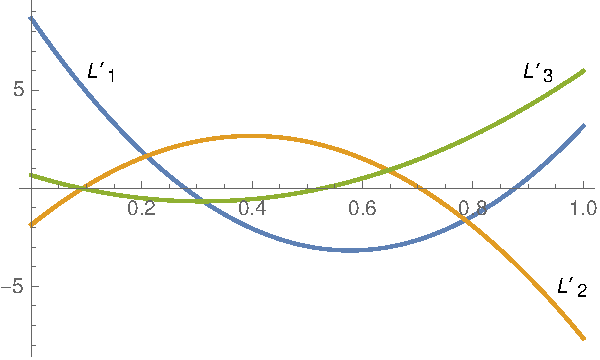
\includegraphics[width=\textwidth]{fig/dl_color.pdf}
		\caption{Производные базисных многочленов. Красным выделены промежутки, на которых выполняется теорема.}
	\end{figure}
	
	\note {
	Так как опорные точки уже известны, построим соответствующие базисные многочлены. На представленном графике показаны графики их производных, а красным выделены участки оси, при нахождении z в которых выполняется условие теоремы. На графике видно свойство, определяющее эти промежутки: на них знаки производных базисных чередуются. То есть полученный план является оптимальным планом для оценки производной в точке z, если z меньше $0.1$, больше $0.9$ или находится на $[0.3, 0.5]$ (все значения приближенные)
	}
\end{frame}

\section{Численное нахождение оптимальных планов}

\begin{frame}
	\frametitle{Численное нахождение оптимальных планов}
	\begin{itemize}
		\item С-оптимальность плана определяется как решение задачи оптимизации
		\item Теорема Элвинга дает критерий С-оптимальности
		\item Поэтому численный алгоритм может быть устроен следующим образом:
		\begin{enumerate}
			\item Численно оптимизируем функцию $\Phi(\xi)$ из определения со случайным начальным планом
			\item Проверяем выполнение условий теоремы Элвинга
			\begin{itemize}
				\item Если они выполнены --- у нас есть результат
				\item Если нет --- возвращаемся к п. 1
			\end{itemize}
		\end{enumerate}
	\end{itemize}
	
	\note {
	Далее рассмотрен алгоритм численного нахождения с-оптимальных планов в общем случае для произвольного $c$. Само определение с-оптимальных планов содержит задачу минимизации, а теорема Элвинга дает критерий того, является ли данный план с-оптимальным. Поэтому очевидным алгоритмом нахождения ответа для данного с будет следующий: найти минимум функции $\Phi$ из определения c-оптимальности с помощью подходящего алгоритма оптимизации со случайной начальной точкой, проверить результат с помощью теоремы Элвинга, и, если критерий выполнен, вывести результат, иначе повторить процедуру. Остаются технические вопросы: как оптимизировать функцию $\Phi(\xi)$ и как проверять теорему Элвинга численно.
	}
\end{frame}

\begin{frame}
	\frametitle {Оптимизация $\Phi(\xi)$}
	\begin{itemize}
		\item У любой матрицы $A^-(x)$ при условии постоянного ранга существует непрерывная вторая производная выражающаяся через производные $A(x)$
		\item Так как $\Phi(\xi) = c^\top M^-(\xi) c$, а ранг $M(\xi)$ зависит только от количества опорных точек, то существуют вторые производные у $\Phi$ по опорным точкам и весам
		\item Поэтому был использован квазиньютоновский алгоритм оптимизации с ограничениями L-BFGS-B 
	\end{itemize}
	
	\note {
	Для оптимизации необходим алгоритм поддерживающий ограничения на область значений (хотя бы типа “коробка”) и который бы сходился с приемлемой скоростью на нашей задаче (потому что возможно, что алгоритм будет множество раз попадать в локальный минимум перед тем, как попадет в глобальный).
	Существует формула, которая выражает в явном виде производную к псевдообращению матрицы А(х), если её ранг не зависит от х (и далее можно перейти ко второй производной). А функция $\Phi$ выражается через псевдообращение информационной матрицы. Поэтому при фиксированном размере плана можно эффективно использовать квазиньютоновские методы оптимизации с ограничениями (здесь использован L-BFGS-B). 

	}
\end{frame}

\begin{frame}
	\frametitle{Проверка условий теоремы Элвинга}
	Нужно найти такой вектор $p$, что $\abs{p^\top f(x)} \leqslant 1$, при этом равенство достигается в опорных точках. Такие $p$ будут решением уравнения
	\begin{equation*}
		\begin{pmatrix}
			f_1(x_1) & \dots & f_n(x_1) \\
			f_1(x_2) & \dots & f_n(x_2) \\
  			\vdots &   \ddots & \vdots \\
  			f_1(x_n)  & \dots & f_n(x_n) \\
  			f'_1(x_{i_1}) & \dots & f'_n(x_{i_1}) \\
  			\vdots &   \ddots & \vdots \\
  			f'_1(x_{i_m})  & \dots & f'_n(x_{i_m})
		\end{pmatrix} 
		p =
		\begin{pmatrix}
			1 \\ s_2 \\ \vdots \\ s_n \\ 0 \\ \vdots \\ 0
		\end{pmatrix},
	\end{equation*}
	где $x_{i_j}$ --- опорные точки не на границе области планирования, а $s_i = \pm 1$.
	
	\note {
	Встает вопрос: как проверять существующий критерий с-оптимальности? По теореме Элвинга должен существовать такой вектор коэффициентов $p$, что его скалярное произведение с регрессионными функциями по модулю не превосходит единицу, а при этом строгое равенство достигается в точках плана. Такой вектор $p$ будет удовлетворять одной из таких систем уравнений: $p^\top f(x)$ равен плюс или минус  единице в данных точках плана (будут перебираться все варианты), а во всех точках плана, лежащих не на границах отрезка, производная функции $p^\top f(x)$ равна нулю, так как в этих точках по определению должен быть локальный экстремум.
	}
\end{frame}

\begin{frame}
	\frametitle{Проверка условий теоремы Элвинга}
	Для всех $p$ с нулевой невязкой для предыдущего уравнения и данного плана $\xi$, проверяем третье условие теоремы Элвинга:
	\begin{equation*}
		c = h \sum_{i=1}^m \omega_i f(x_i) p^\top f(x_i)
	\end{equation*}
	
	\begin{itemize}
		\item Для того, чтобы не вычислять $h$ достаточно проверять коллинеарность векторов
		\item Все сравнения с точностью до машинного нуля
		\item Если равенство выполняется, то $\xi$ --- с-оптимальный план
	\end{itemize}
	
	\note {
	Взяв все такие $p$, невязка которых с предыдущим уравнением равна нулю, можно проверять третье условие теоремы Элвинга, которое выглядит как следующее равенство, в котором известно всё, кроме константы h, нахождение которой можно опустить, так как ясно, что она существует, если вектора в левой и правой части коллинеарны. Произведя все сравнения с точностью до машинного нуля, выполнение этого равенства для уже найденного вектора $p$ и данного плана $\xi$ равносильно тому, что план $\xi$ является с-оптимальным, а иначе --- не является. 
	Таким образом процедура нахождения с-оптимальных планов в общем случае построена.
	}
\end{frame}


\begin{frame}
	\frametitle{Результаты}
	\begin{itemize}
		\item Описаны оптимальные планы размера $n$ для нахождения производной в полиномиальной модели без свободного члена с $\mathcal{X} = [0, 1]$
		\item Приведен пример применения этого результата
		\item Разработан алгоритм численного нахождения с-оптимальных планов в общем случае
	\end{itemize}
	
	\note {
	В работе на текущий момент были описаны некоторые явные решения для нахождения планов для оценки производной в модели без нулевого члена, рассмотрен пример применения полученных результатов и построен алгоритм нахождения с-оптимальных планов в общем случае.
	}
\end{frame}

	\nobibliography{diploma}

\end{document}